% Arreglo 3x3x3 del símbolo de Levi-Civita (libro fig. 1.5)
% Proyección isométrica: (i,j,k) -> ( i + 0.5k , -j + 0.4k )
\documentclass[border=6pt]{standalone}
\usepackage{tikz}
\usetikzlibrary{arrows.meta}
\begin{document}
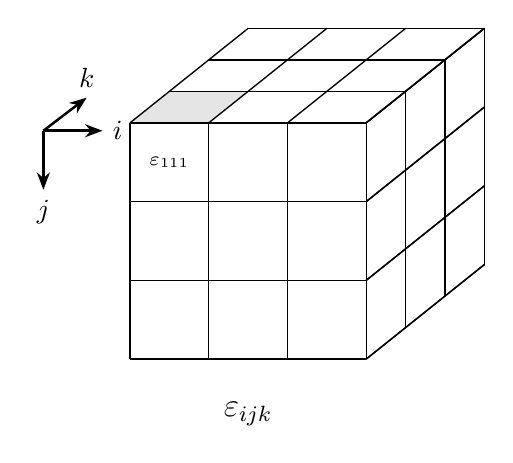
\begin{tikzpicture}[line width=0.5pt, >={Stealth[length=2.2mm]}]
  % celda destacada (frente, esquina superior izquierda): epsilon_111
  \fill[black!10] ({0+0.5*0},{-0+0.4*0}) -- ({1+0.5*0},{-0+0.4*0})
                  -- ({1+0.5*1},{-0+0.4*1}) -- ({0+0.5*1},{-0+0.4*1}) -- cycle;
  % --- cara frontal (k=0): plano i-j ---
  \foreach \i in {0,1,2,3} { \draw ({\i},{0}) -- ({\i},{-3}); }
  \foreach \j in {0,1,2,3} { \draw ({0},{-\j}) -- ({3},{-\j}); }
  % --- cara superior (j=0): plano i-k ---
  \foreach \i in {0,1,2,3} { \draw ({\i},{0}) -- ({\i+1.5},{1.2}); }
  \foreach \k in {0,1,2,3} { \draw ({0+0.5*\k},{0.4*\k}) -- ({3+0.5*\k},{0.4*\k}); }
  % --- cara derecha (i=3): plano j-k ---
  \foreach \j in {0,1,2,3} { \draw ({3+0.5*\j*0+3*0},{-\j}) -- ({3+1.5},{-\j+1.2}); }
  \foreach \j in {0,1,2,3} { \draw ({3},{-\j}) -- ({3+1.5},{-\j+1.2}); }
  \foreach \k in {0,1,2,3} { \draw ({3+0.5*\k},{0+0.4*\k}) -- ({3+0.5*\k},{-3+0.4*\k}); }
  % ejes (triada): i derecha, j abajo, k profundidad
  \draw[->, line width=0.9pt] (-1.1,-0.1) -- (-0.35,-0.1) node[right]{$i$};
  \draw[->, line width=0.9pt] (-1.1,-0.1) -- (-1.1,-0.85) node[below]{$j$};
  \draw[->, line width=0.9pt] (-1.1,-0.1) -- ({-1.1+0.55},{-0.1+0.42}) node[above]{$k$};
  % etiquetas
  \node at ({0.5},{-0.5}) {\scriptsize$\varepsilon_{111}$};
  \node[font=\large] at (1.5,-3.7) {$\varepsilon_{ijk}$};
\end{tikzpicture}
\end{document}
